\section{Results}\label{sec:results}

\begin{figure*}
    \centering
    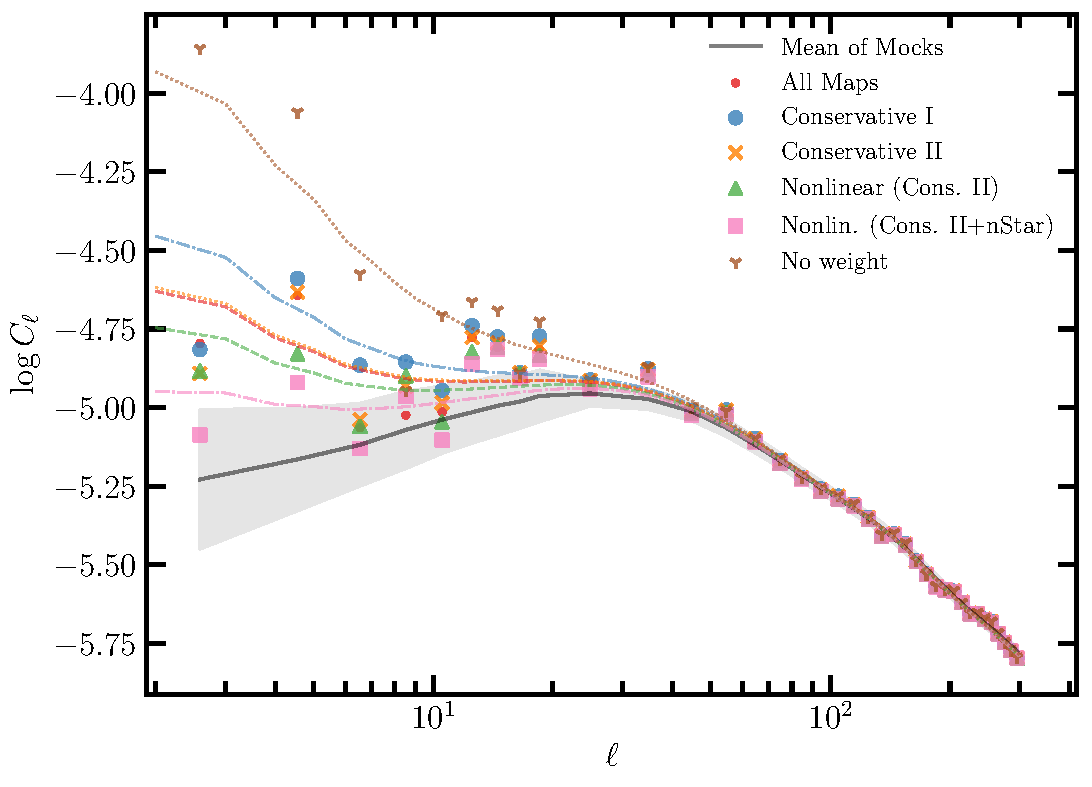
\includegraphics[width=0.9\textwidth]{figures/model_dr9.pdf} 
    \caption{The angular power spectrum of the DESI LRG targets before (\textit{No weight}) and after correcting for imaging systematics using the linear and non-linear methods with their corresponding best-fitting theory curves. The solid curve and grey shade respectively represent the mean power spectrum and $68\%$ error from the $\fnl=0$ mocks.}
    \label{fig:cl_dr9}
\end{figure*}

This section presents our $\fnl$ constraints from the DESI LRG targets. The analysis is not carried out blindly. However, the cleaning methods are decided only based on the cross power spectrum and mean density contrast statistics. \mr{Alex: Might be nice to have a table listing all cleaning methods used—since there are more than just the 3 map combinations in 2.1.2} \mr{Edmond: Fig12: DESI is : you compute the Cl on all the footprint? it is not a combination of the independent measurement of the three regions? same remark for the other figures/tabs.} \mr{Ashley: explain how the data is combined.} \mr{Ashley: I think text on blinding could be more like "Our fiducial choice of the 3 map method and robustness tests on (list whatever would make sense at this point) were applied to the data to obtain fNL constraints with no mitigation bias correction and first without revealing the fNL values of the posterior likelihoods (only their relative shifts). After we chose the 3 map method as our fiducial method, we applied further robustness tests and derived the mitigation bias correction."}

\subsection{DESI imaging LRG sample}
Figure \ref{fig:cl_dr9} shows the measured power spectrum of the DESI LRG targets before and after applying imaging weights and the best-fitting theory curves. The solid line and the grey shade represent respectively the mean power spectrum and 1$\sigma$ error, estimated from the $\fnl=0$ lognormal simulations. The differences between various cleaning methods are significant on large scales ($\ell > 20$), but the small scale clustering measurements are consistent. By comparing \textit{linear two maps} to \textit{linear three maps}, we find that the measured clustering power on modes with $6\leq \ell < 10$ are noticeably different between the two methods. We associate the differences to the additional map for psfsize in the r-band, which is included in \textit{linear three maps}. On other scales, the differences between \textit{linear three maps} and \textit{linear eight maps} are negligible, supporting the idea that our feature selection procedure has been effective in identifying the primary maps which cause the large-scale excess clustering signal. Comparing \textit{non-linear three maps} to \textit{linear three maps}, we find that the measured spectra on $4 \leq \ell < 6$ are very different, probably indicating some non-linear spurious fluctuations with large scale characteristics due to extinction. Including stellar density in the non-linear approach (\textit{non-linear four maps}) further reduces the excess power relative to the mock power spectrum, in particular on modes between $2\leq \ell < 4$. However, when calibrated on the lognormal simulations, we find that these differences are reversed after accounting for over-correction. Therefore, we associate the subtraction after $nStar$ to over fitting.


\subsubsection{Calibrated constraints}

\begin{figure}
    \raggedleft
    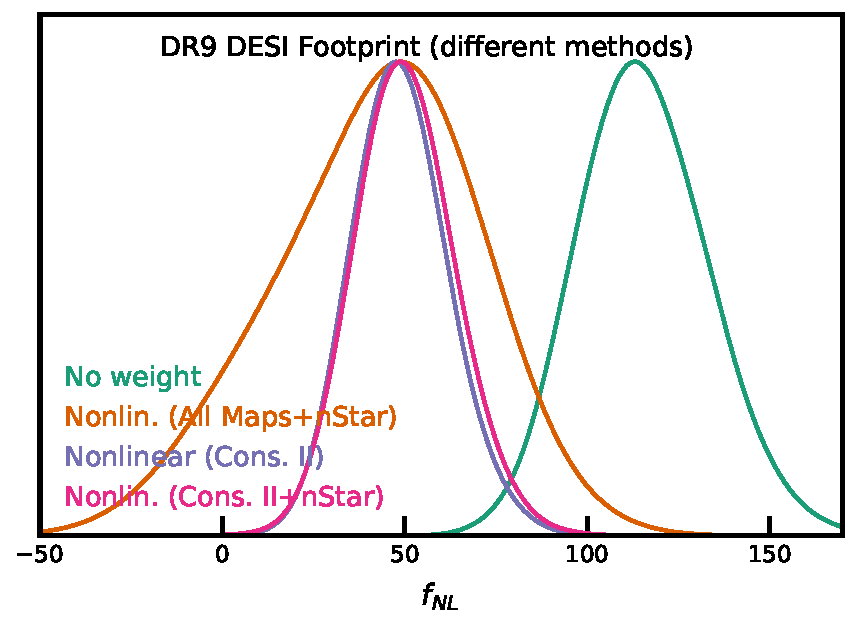
\includegraphics[width=0.435\textwidth, trim={0 1.4cm 0 0},clip]{mcmc_dr9methods1d.pdf}
    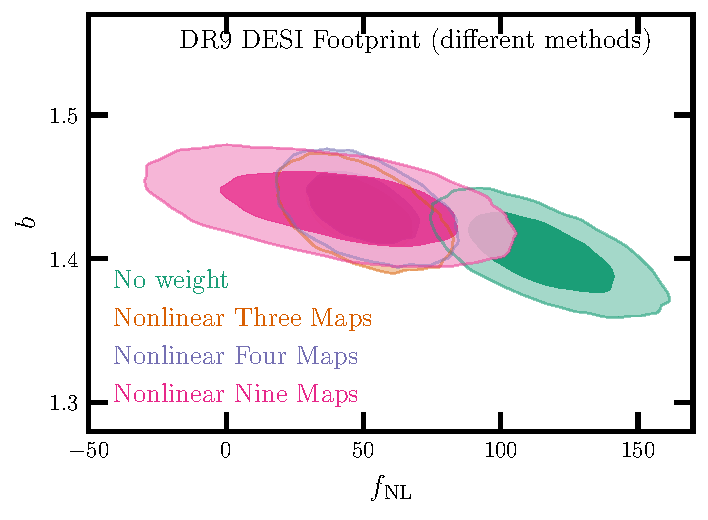
\includegraphics[width=0.46\textwidth, trim={0 0 0.15cm 0.2cm},clip]{figures/mcmc_dr9methods.pdf} 
    \caption{The calibrated constrains from the DESI LRG targets. \textit{Top}: probability distribution for $\fnl$ marginalized over the shotnoise and bias. \textit{Bottom}: $68\%$ and $95\%$ probability distribution contours for the bias and $\fnl$ from the DESI LRG targets before and after applying non-linear cleaning methods. The lognormal mocks are used to calibrate these distributions for over correction.}\label{fig:mcmc_dr9}
\end{figure}

\begin{table*}
    \caption{The calibrated best-fitting, marginalized mean, and marginalized $68\%$ ($95\%$) confidence estimates for $\fnl$ from fitting the power spectrum of the DESI LRG targets before and after correcting for imaging systematic effects.}
    \label{tab:dr9methodcalib}
   \centerline{%     
    \begin{tabular}{llllllll}
    \hline
    \hline
   &  & 	  & & $\fnl$ &  &  \\
   \cmidrule(r{.7cm}){3-6}
Footprint                               & Method & 	Best fit  & Mean & $ 68\%$ CL & $ 95\%$ CL & $\chi^{2}$/dof \\
    \hline
DESI                      & No Weight   & $113.18$& $115.49$& $ 98.14<\fnl<132.89$& $ 83.51<\fnl<151.59$ &   44.4/34\\
DESI                      & Nonlinear Three Maps& $ 47.38$& $ 48.81$& $ 36.08<\fnl< 61.44$& $ 25.03<\fnl< 75.64$ &   34.6/34\\
DESI                      & Nonlinear Four Maps& $ 48.92$& $ 50.10$& $ 36.88<\fnl< 63.31$& $ 24.87<\fnl< 77.78$ &   35.2/34\\
DESI                      & Nonlinear Nine Maps& $ 49.69$& $ 41.91$& $ 13.10<\fnl< 69.14$& $-15.96<\fnl< 91.84$ &   39.5/34\\
   \hline
    \end{tabular}
}
\end{table*}

All $\fnl$ constraints presented here are calibrated for the effect of over correction using the lognormal simulations. Table \ref{tab:dr9methodcalib} describes the best-fitting and marginalized mean estimates of $\fnl$ from fitting the power spectrum of the DESI LRG targets before and after cleaning with the non-linear approach given various combinations for the imaging systematic maps. Figure \ref{fig:mcmc_dr9} shows the marginalized probability distribution for $\fnl$ in the top panel, and the $68\%$ and $95\%$ probability contours for the linear bias parameter and $\fnl$ in the bottom panel, from our sample before and after applying various corrections for imaging systematics. Overall, we find the maximum likelihood estimates to be consistent among the various cleaning methods. We obtain $36.08 (25.03) < \fnl < 61.44(75.64)$ with $\chi^{2}=34.6$ for \textit{non-linear three maps} over 34 degrees of freedom. Accounted for over-correction, we obtain $36.88(24.87) < \fnl < 63.31(77.78)$ with $\chi^{2}=35.2$ with the additional stellar density map in the \textit{non-linear four maps}. With or without $nStar$, the confidence intervals are consistent with each other and more than $3\sigma$ off from zero PNG. Cleaning the sample with \textit{non-linear nine maps} weakens our constraints to $13.10(-15.96) < \fnl < 69.14(91.84)$ with $\chi^{2}=39.5$. For comparison, we obtain $98.14(83.51) < \fnl < 132.89(151.59)$ at $68\% (95\%)$ confidence with $\chi^{2}=44.4$ for the \textit{no weight} approach.

\subsubsection{Uncalibrated constraints: robustness tests}
\mr{Alex: I may have missed this—but do you ever quote the marginalized fnl constraints without mitigation bias (corresponding to Fig. 12)? I think they should probably be in a table and commented on in the text.
}  

\mr{Figure \ref{fig:mcmcdr9noshift} shows the probability distributions of $\fnl$ for various treatments before accounting for the over-correction effect. The method with the largest flexibility and more number of imaging systematic maps is more likely to regress out the clustering signal and return biased $\fnl$ constraints. As expected, non-linear nine maps yields a smaller maximum likelihood estimate of $\fnl$. Our non-linear three maps returns a best-fitting estimate of $\fnl=26$ with the $68\%(95\%)$ confidence of $19(9)<\fnl <41(53)$ and $\chi^{2}=34.6$. With the stellar density map included, non-linear four maps yields a smaller best-fitting estimates of $\fnl=17$ with the error of $7(-2)<\fnl<27(38)$. The non-linear nine maps gives an asymetric posterior with the marginalized mean $\fnl=-9$, best estimate $\fnl=-6$ with the error of $-21(-34)<\fnl<2.4(12)$.}

Now we proceed to perform some robustness tests and assess how sensitive the $\fnl$ constraints are to the assumptions made in the analysis or the quality cuts applied to the data. For each case, we re-train the cleaning methods and derive new sets of imaging weights. Accordingly, for the cases where a new survey mask is applied to the data, we re-calculate the covariance matrices using the new survey mask to account for the changes in the survey window and integral constraint effects. Calibrating the mitigation biases for all of these experiments is beyond the scope of this work and redundant, as we are only interested in the relative shift in the $\fnl$ constraints after changing the assumptions. Therefore, the absolute scaling of the $\fnl$ constraints presented here are biased because of the over correction effect. Table \ref{tab:dr9method} summarizes the uncalibrated $\fnl$ constraints from the DESI LRG targets. Our tests are as follows:

\begin{table*}
    \caption{The uncalibrated best-fitting and marginalized mean estimates for $\fnl$ from fitting the power spectrum of the DESI LRG targets before and after correcting for systematics. The estimates are not calibrated for over correction, and thus are subject to mitigation systematics. The number of degrees of freedom is 34 (37 data points - 3 parameters). The lowest mode is $\ell=2$ and the covariance matrix is from the $\fnl=0$ clean mocks (no mitigation) except for the case with '+cov' in which the covariance matrix is from the $\fnl=76.9$ clean mocks (no mitigation).}
    \label{tab:dr9method}
   \centerline{%     
    \begin{tabular}{llllllll}
    \hline
    \hline
   &  & 	  & & $\fnl$ + Mitigation Systematics &  &  \\
   \cmidrule(r{.7cm}){3-6}
Footprint                               & Method & 	Best fit  & Mean & $ 68\%$ CL & $ 95\%$ CL & $\chi^{2}$ \\
    \hline
DESI                      & No Weight   & $113.18$& $115.49$& $ 98.14<\fnl<132.89$& $ 83.51<\fnl<151.59$ &   44.4\\
DESI                      & Linear Eight Maps& $ 36.05$& $ 37.72$& $ 26.13<\fnl< 49.21$& $ 16.31<\fnl< 62.31$ &   41.1\\
DESI                      & Linear Two Maps& $ 49.58$& $ 51.30$& $ 38.21<\fnl< 64.33$& $ 27.41<\fnl< 78.91$ &   38.8\\
DESI                      & Linear Three Maps& $ 36.63$& $ 38.11$& $ 26.32<\fnl< 49.86$& $ 16.36<\fnl< 63.12$ &   39.6\\
DESI                      & Nonlinear Three Maps& $ 28.58$& $ 29.79$& $ 18.91<\fnl< 40.59$& $  9.47<\fnl< 52.73$ &   34.6\\
DESI (imag. cut)          & Nonlinear Three Maps& $ 29.16$& $ 30.57$& $ 19.05<\fnl< 42.18$& $  9.01<\fnl< 54.81$ &   35.8\\
DESI (comp. cut)          & Nonlinear Three Maps& $ 28.07$& $ 29.48$& $ 18.38<\fnl< 40.50$& $  8.81<\fnl< 53.10$ &   34.5\\
DESI                      & Nonlinear Four Maps& $ 16.63$& $ 17.52$& $  7.51<\fnl< 27.53$& $ -1.59<\fnl< 38.49$ &   35.2\\
DESI                      & Nonlinear Nine Maps& $ -5.87$& $ -9.19$& $-21.45<\fnl<  2.40$& $-33.81<\fnl< 12.06$ &   39.5\\
DESI                     & Nonlinear Three Maps+$f_{\rm NL}=76.92$ Cov& $ 31.62$& $ 33.11$& $ 20.94<\fnl< 45.24$& $ 10.56<\fnl< 59.16$ &   33.5\\
\hline
BASS+MzLS                 & Nonlinear Three Maps& $ 15.43$& $ 19.01$& $ -1.17<\fnl< 39.43$& $-19.19<\fnl< 63.56$ &   35.6\\
BASS+MzLS                 & Nonlinear Four Maps& $ 13.12$& $ 15.39$& $ -4.59<\fnl< 35.56$& $-24.88<\fnl< 59.31$ &   34.7\\
BASS+MzLS                 & Nonlinear Nine Maps& $ -3.73$& $ -6.34$& $-27.11<\fnl< 13.75$& $-47.44<\fnl< 33.94$ &   36.8\\
BASS+MzLS (imag. cut)     & Nonlinear Three Maps& $ 25.03$& $ 29.12$& $  6.16<\fnl< 52.44$& $-14.22<\fnl< 80.54$ &   36.2\\
BASS+MzLS (comp. cut)     & Nonlinear Three Maps& $ 16.99$& $ 20.90$& $  0.26<\fnl< 41.76$& $-18.30<\fnl< 67.12$ &   35.8\\
DECaLS North              & Nonlinear Three Maps& $ 41.02$& $ 44.89$& $ 23.33<\fnl< 66.78$& $  4.96<\fnl< 93.02$ &   41.1\\
DECaLS North              & Nonlinear Four Maps& $ 31.45$& $ 34.78$& $ 14.14<\fnl< 55.79$& $ -5.81<\fnl< 80.80$ &   41.2\\
DECaLS North              & Nonlinear Five Maps& $ 55.46$& $ 60.44$& $ 36.78<\fnl< 84.05$& $ 17.86<\fnl<112.81$ &   38.4\\
DECaLS North              & Nonlinear Nine Maps& $  0.81$& $ -5.68$& $-29.73<\fnl< 16.71$& $-53.15<\fnl< 36.19$ &   45.1\\
DECaLS North (no DEC cut) & Nonlinear Three Maps& $ 41.05$& $ 44.82$& $ 23.58<\fnl< 66.08$& $  6.40<\fnl< 91.42$ &   40.7\\
DECaLS North (imag. cut)  & Nonlinear Three Maps& $ 43.27$& $ 48.39$& $ 24.60<\fnl< 72.50$& $  4.71<\fnl<101.42$ &   35.1\\
DECaLS North (comp. cut)  & Nonlinear Three Maps& $ 40.55$& $ 44.63$& $ 22.41<\fnl< 67.11$& $  3.95<\fnl< 94.06$ &   41.4\\
DECaLS South              & Nonlinear Three Maps& $ 31.24$& $ 33.21$& $ 14.89<\fnl< 52.40$& $ -5.11<\fnl< 74.35$ &   30.2\\
DECaLS South              & Nonlinear Four Maps& $ 14.34$& $  6.28$& $-21.19<\fnl< 30.01$& $-53.63<\fnl< 49.51$ &   31.9\\
DECaLS South              & Nonlinear Five Maps& $ 33.79$& $ 37.50$& $ 17.71<\fnl< 57.42$& $ -0.31<\fnl< 80.94$ &   30.8\\
DECaLS South              & Nonlinear Nine Maps& $-36.76$& $-32.01$& $-49.38<\fnl<-13.61$& $-65.26<\fnl<  7.52$ &   31.5\\
DECaLS South (no DEC cut) & Nonlinear Three Maps& $ 43.79$& $ 46.79$& $ 30.16<\fnl< 63.41$& $ 16.38<\fnl< 82.72$ &   23.8\\
DECaLS South (imag. cut)  & Nonlinear Three Maps& $ 26.47$& $ 23.36$& $  3.18<\fnl< 47.84$& $-57.69<\fnl< 71.39$ &   30.0\\
DECaLS South (comp. cut)  & Nonlinear Three Maps& $ 29.62$& $ 31.76$& $ 13.00<\fnl< 51.58$& $ -9.78<\fnl< 74.28$ &   29.7\\
   \hline
    \end{tabular}}
\end{table*}
\begin{figure}
    \centering
    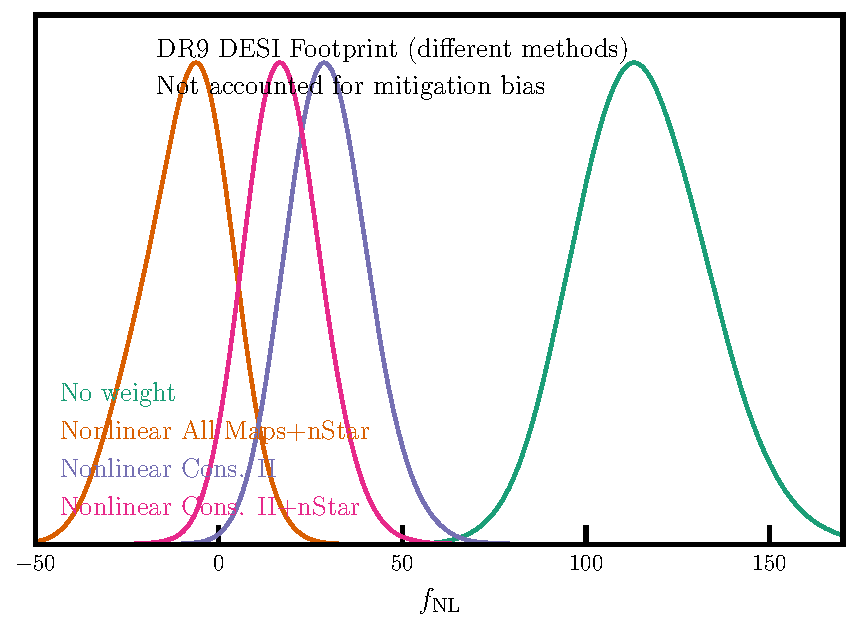
\includegraphics[width=0.45\textwidth]{figures/mcmc_dr9methods1dnoshift.pdf}
    \caption{Same as Figure \ref{fig:mcmc_dr9} but without accouting for over correction. }
    \label{fig:mcmcdr9noshift}
\end{figure}
\begin{figure}
    \centering
    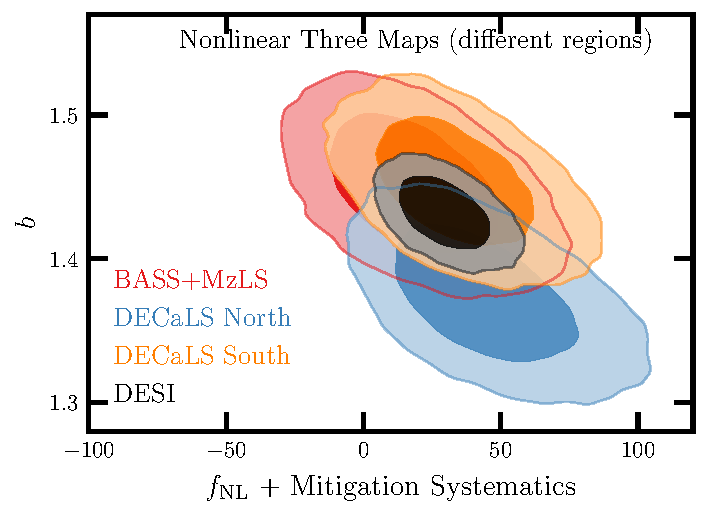
\includegraphics[width=0.45\textwidth]{figures/mcmc_dr9regions.pdf} 
    \caption{The uncalibrated 2D constraints from the DESI LRG targets for each imaging survey compared with that for the whole DESI footprint. The dark and light shades represent the $68\%$ and $95\%$ confidence intervals, respectively. \mr{Edmond: maybe comment why the bias is lower in Decals-north? Have you a physical explanation?}}\label{fig:mcmc_dr9reg}
\end{figure}
\begin{figure*}
    \centering
    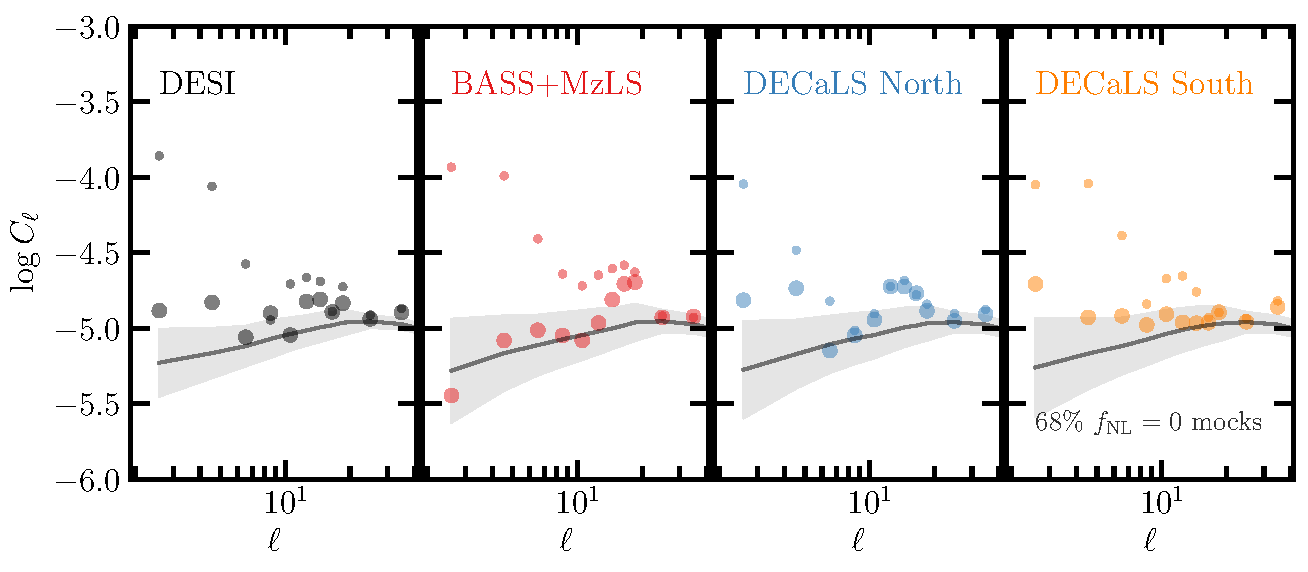
\includegraphics[width=0.85\textwidth]{figures/cldr9_lowell.pdf}
    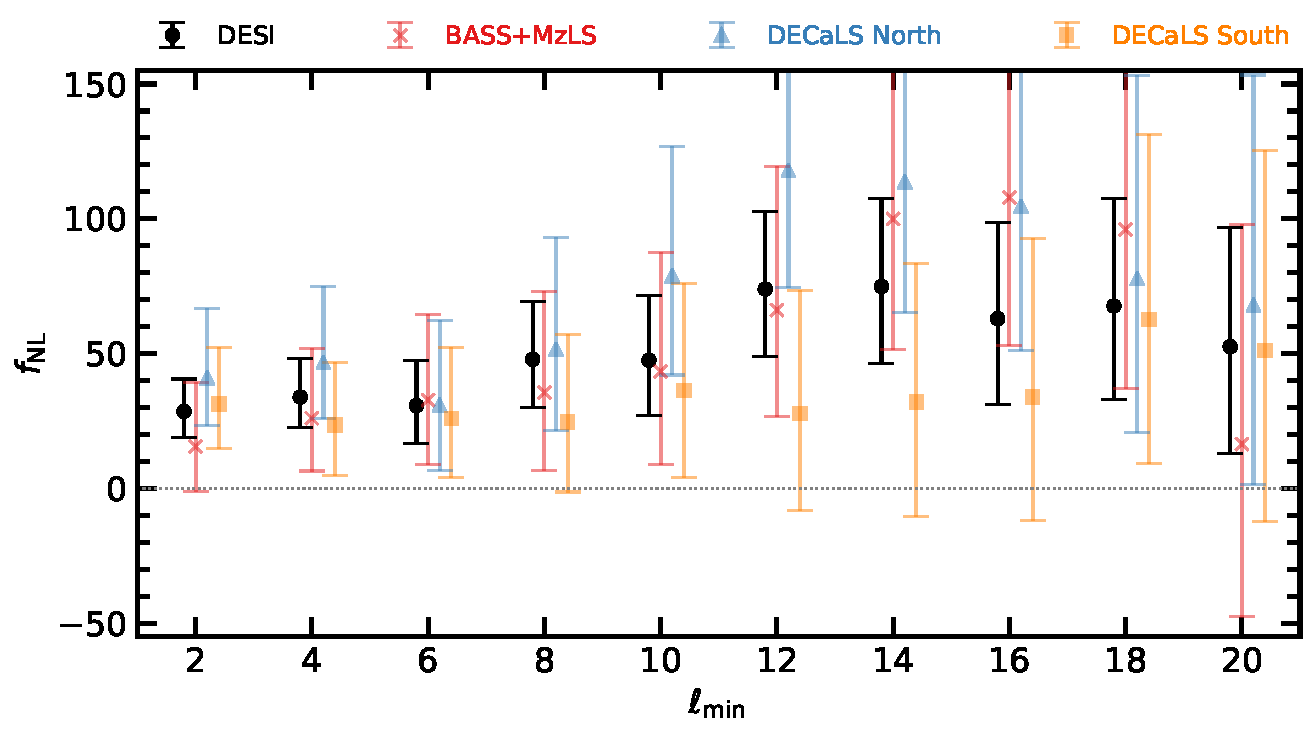
\includegraphics[width=0.86\textwidth]{figures/fnl_elmin.pdf}  
    \caption{\mr{Top: The measured power spectrum of the DESI LRG targets before (solid curves) and after \textit{non-linear three maps} (scatter points) for the DESI, BASS+MzLS, DECaLS North, and DECaLS South regions. Bottom: The uncalibrated $\fnl$ constraints vs the lowest $\ell$ mode used for fitting $\fnl$. The points represent marginalized mean estimates of $\fnl$ and error bars represent $68$\% confidence estimated from the $\fnl=0$ mocks. The scaling of $\fnl$ is not calibrated to account for over correction caused by mitigation.}}\label{fig:mcmc_dr9elmin}
\end{figure*}

\begin{itemize}[itemindent=*]

\item \textbf{Linear methods}: We find consistent constraints from \textit{linear eight maps} and \textit{linear three maps}, $26(16)<\fnl<49(62)$ vs $26(16)<\fnl<50(63)$ at $68\%(95\%)$ confidence, which suggests that not all of the eight imaging systematic maps are needed to completely mitigate systematic effects. \mr{ADD how this compares to nonlinear constraints.}

\item \textbf{Imaging regions}: We compare how our constraints from fitting the power spectrum of the whole DESI footprint compares to that from the power spectrum of each imaging region individually, namely BASS+MzLS, DECaLS North, and DECaLS South. Figure~\ref{fig:mcmc_dr9reg} shows the $68\%$ and $95\%$ probability contours on $\fnl$ and $b$ from each individual region, compared with that from DESI. The cleaning method here is \textit{non-linear three maps}, and the covariance matrices are estimated from the $\fnl=0$ mocks. Overall, we find that the constraints from all imaging surveys are consistent with each other and DESI within $68\%$ confidence. Ignoring the over-correction effect, both BASS+MzLS and DECaLS South yield constraints consistent with $\fnl=0$ within $95\%$, but DECaLS North deviates from zero PNG at more than $2\sigma$. This motivates follow-up studies with the spectroscopic sample of LRGs in DECaLS North. \mr{Edmond: maybe comment why the bias is lower in Decals-north? Have you a physical explanation?} \mr{Ashley: The statement about DECaLS north being the region with the most significantly non-zero fNL was a little confusing. I would re-write to something like: "Ignoring the over-correction effect, we find that the results from the DECaLS North region to be the only one that finds PNG nonzero at greater than 95\%."}

\item \textbf{Stellar density template (\textit{nStar})}: Adding the stellar density template (\textit{non-linear four maps}) does not change the constraints from BASS+MzLS much, but it shifts the $\fnl$ distributions to lower values in DECaLS North and DECaLS South by $0.5\sigma$ and $\sigma$, respectively, reconciling all constraints with $\fnl=0$. We note that differences are more significant when all nine maps are used as input. This is somewhat expected as cleaning the data with more imaging systematic maps is more prone to the over-correction issue. \mr{We find that the shifts in $\fnl$ from adding $nStar$ are reveresed after accounting for the over correction effect. Comparing the $\fnl$ constraints from \textit{non-linear four maps} and \textit{non-linear three maps} in Table \ref{tab:dr9methodcalib} to those in \ref{tab:dr9method}, we can argue that the $\fnl$ shifts after adding $nStar$ are probably caused by the over-correction issue from the chance correlations between the stellar density map and large-scale structure.} \mr{Ashley: When not accounting for mitigation bias, adding the stellar density map appears to result in significant changes, but these changes go away when we account for the mitigation bias and we find all methods recover the same maximum likelihood estimate for fNL to within XX} 

\item \textbf{Pixel completeness (\textit{comp. cut})}: We discard pixels with fractional completeness less than half to assess the effect of partially complete pixels on $\fnl$. This cut removes $0.6\%$ of the survey area, and no changes in the $\fnl$ constraints are observed.

\item \textbf{Imaging quality (\textit{imag. cut})}: Pixels with poor photometry are removed from our sample by applying the following cuts on imaging; $E[B-V]<0.1$, $nStar < 3000$, ${\rm depth}_{g} > 23.2$, ${\rm depth}_{r} > 22.6$, ${\rm depth}_{z} > 22.5$, ${\rm psfsize}_{g}<2.5$, ${\rm psfsize}_{r}<2.5$, and ${\rm psfsize}_{z}<2$. Although these cuts remove $8\%$ of the survey mask, there is a negligible impact on the best-fitting $\fnl$ from fitting the DESI power spectrum. However, when each region is fit individually, the BASS+MzLS constraint shift toward higher values of $\fnl$ by approximately $\Delta \fnl \sim 10$, whereas the constraints from DECaLS North and DECaLS South do not change significantly. 

e\item \textbf{Covariance matrix (\textit{cov})}: We fit the power spectrum of our sample cleaned with \textit{non-linear three maps} correction, but use the covariance matrix constructed from the $\fnl=76.92$ mocks. With the alternative covariance, a $12\%$ increase in the $\sigma \fnl$ is observed. We also find that the best-fitting and marginalized mean estimates of $\fnl$ increase by $10-11\%$. Overall, we find that the differences are not significant in comparison to the statistical precision.

\item \textbf{External maps (\textit{CALIBZ+HI})}: The neural network five maps correction includes the additional maps for HI and CALIBZ. With this correction, the best-fitting $\fnl$ increases from $41.02$ to $55.46$ for DECaLS North and from $31.24$ to $33.79$ for DECaLS South, which might suggest that adding HI and CALIBZ increases the input noise, and thus negatively impacts the performance of the neural network model. This test is not performed on BASS+MzLS due to a lack of coverage from the CALIBZ map. 

\item \textbf{Declination mask (\textit{no DEC cut})}: The fiducial mask removes the disconnected islands in DECaLS North and regions with DEC $<-30$ in DECaLS South, where there is a high likelihood of calibration issues as different standard stars are used for photometric calibrations. We analyze our sample without these cuts, and find that the best-fitting and marginalized $\fnl$ mean estimates from DECaLS South shift significantly to higher values of $\fnl$ by $\Delta \fnl \sim 10$, which supports the issue of photometric systematics in the DECaLS South region below DEC $=-30$. On the other hand, the constraints from DECaLS North do not change significantly, indicating the islands do not induce significant contaminations. \bbk{[Did you try cutting out more of DECaLS North, such as everything below the equator?]}

\item \textbf{Scale dependence (\textit{varying $\ell_{\rm min}$})}: We raise the value of the lowest harmonic mode $\ell_{\rm min}$ used for the likelihood evaluation during MCMC. This is equivalent to decreasing the highest scale of measurement in the power spectrum. By doing so, we anticipate a reduction in the impact of imaging systematics on $\fnl$ inference as lower $\ell$ modes are more likely to be contaminated. Figure \ref{fig:mcmc_dr9elmin} illustrates the power spectra before and after the correction with \textit{non-linear three maps} in the top panel. The bottom panel shows the marginalized mean and $68\%$ error on $\fnl$ with \textit{non-linear three maps} for the DESI, BASS+MzLS, DECaLS North, and DECaLS South regions. \mr{ALEX: We find that the mean estimates of $\fnl$ slightly shifts to higher values on scales $12<\ell<18$ in DECaLS North and BASS+MzLS when higher $\ell_{\rm min}$ is used. This is the opposite behavior from what one would expect if there were just a giant systematics induced spike at low $\ell$. So it shows that the issue here is more subtle than what one would have initially suspected.} \mr{Edmond: Fig10 / 13: do you have an explanation why there is this remaining bump at l=10-12 ?? is a correction artefact ? you should mention it in the text and comment the effect since it increase the value of fnl when you chose higher $l_min$.}

\end{itemize}

\subsection{Summary}
In summary, we find that the non-linear methods outperform the linear methods in removing the excess clustering signal on large scales. Adding the stellar density map results in significant changes, however when accounted for the mitigation bias, all methods recover the same maximum likelihood estimate. With calibration on the lognormal mocks, the neural network three maps and four maps approaches show $\fnl$ detection at more than $2\sigma$ confidence. The most flexible neural network method with nine maps returns a greater associated uncertainty which is consistent with $\fnl=0$. 

We also run various tests with cuts on the DR9 sample or changing the configuration or details of the analysis. Overall, we find consistent results across sub imaging surveys within DESI. However, our results show that a declination cut at DEC $=-30$ is necessary for DECaLS South to avoid potential calibration issues. Our analysis does not show a statistical demand for including external templates for HI and CALIBZ, using a different covariance matrix, or imposing additional cuts on the DR9 sample based on imaging and pixel completeness. We also obtain robust results regardless of the largest scale used for constraining $\fnl$.

\mr{Ashley: I think we need some kind of discussion section for the results. We should also compare the results to those from other galaxy/QSO samples and Planck. If we don't have enough for a whole section, the Conclusions could just become Discussion and Conclusion. I would start the section something like: "We have measured the PNG parameter fNL using the angular clustering of an LRG sample selected from DESI imaging data. In our fiducial analysis, we have found nonzero PNG at XX\% confidence, with a maximum likelihood value of fNL=XX. We have applied a series of robustness tests on the impact of how we estimate the selection function of our LRG sample, including: the methods (), the set of maps used (), and data quality cuts on the accepted regions. We find no change in the analysis that shifts the maximum likelihood value of fNL to a significantly lower value. The only manner in which the significance of nonzero PNG decreases is due to the uncertainty on the measurement increasing when we employ more maps to the selection function estimation and by doing so remove large-scale clustering information (the effect of which on fNL recovery we have calibrated with mocks).}

\mr{We compare our fiducial results to recent CMB and QSO measurements. Assess agreement. If we are in reasonable agreement with QSO measurement, what is combined constraint Either we have measured an fNL signal that is inconsistent with CMB measurements or there is a hidden source of systematic contamination in our data. Discuss generic effect of calibration. Ask Rongpu if we can include the Gaia calibration test map, which shows patterns that look related to the Gaia scanning strategy, rather that Legacy Survey? (If not, we can just say something like "internal DESI tests of the photometric calibration are unable to uncover DESI-specific issues, e.g., when comparing to Gaia data") Then, something like "The most significant trends that we find are with the E(B-V) map. The source of such a trend would be a mis-calibration of the E(B-V) map itself or the coefficients applied to obtain Galactic extinction corrected photometry. Such issues are generically likely to be proportional in amplitude to the estimated E(B-V), but may not strictly follow the estimated E(B-V). In order to explain the fNL signal we measure, such an effect would need to be approximately twice that of the trend we find with E(B-V). There are ongoing efforts within DESI to obtain improved Galactic extinction information, which will help discover if this is indeed the cause. (Anything to say about Mudur et al. map? I think we need to write something. Perhaps for now just something like "a first look at the Mudur et al E(B-V) maps did not suggest including them would change our results" and then during CWR you could add Mudur-SFD as a map to test against?)"}